\section{Zielsetzung}
Das Ziel dieses Versuches ist es, mittels Tomographie als bildgebendes Verfahren, die Zusammensetzung von Würfeln verschiedener Materialien zu untersuchen.
Dabei werden über die Licht-Materie-Wechselwirkung der $\gamma$-Strahlung verschiedene Spektren aufgenommen, die analysiert werden.
	
\section{Theorie}

\noindent
Die Tomopgraphie allgemein ist ein bildgebendes Verfahren, bei dem räumliche Strukturen eines dreidimensionalen Körpers durch Querschnittsbilder untersucht werden.
Dabei wird der Körper mit $\gamma$-Strahlung beschossen. Aus den transmitierten Intensitäten und der Startintensität $I_0$ lassen sich dann Rückschlüsse auf die Zusammensetzung des Körpers schließen.
Unterschiedliche Materialien besitzen nämlich unterschiedliche Absorptionskoeffizienten $\mu_0$, weswegen sie unterschiedlich viel Strahlung absorbieren.\\
Wenn ein Körper dann unter verschiedenen Winkeln bestrahlt wird, wodurch unterschiedliche Projektionen erhalten werden, lässt die Summe der Messungen Folgerungen über die dreidimensionale Zusammensetzung zu.\\
Für die Absorption von Strahlung in Materie beschreibt das Beer-Lambertsche-Gesetz die transmitierte Intensität $I$ im Verhältnis zur Anfangsintensität $I_0$.
\begin{equation}
    I = I_0 \t{exp}\left(- \sum_{i=1}^N \mu_i d_i\right)
    \label{eqn:abs}
\end{equation}
Dabei ist $\mu_i$ der materialspezifische Absorptionskoeffizient des $i$-ten Materials und $d_i$ die Schichtdicke dieses Materials.\\
Dies lässt sich dann für unterschiedliche Projektionen zu einem linearen Gleichungssystem umformen. 
Dafür wird Gleichung \ref{eqn:abs} nach den Absorptionskoeffizienten und den Dicken umgestellt.
\begin{align}
    \ln\left(\frac{I_0}{I}\right) &= \sum_{i=1}^N \mu_i d_i \label{eqn:ln}\\
    \intertext{Dies lässt sich dann in Matrixscheibweise als }
    \vec I &=\left(A^T  A\right)^{-1} A^T \vec \mu
    \label{eqn:mu}
\end{align}
schreiben. Dabei setzt sich $\vec I$ aus den gemessenen Intensitäten des transmitierten Lichts zusammen, $\vec \mu$ aus den Absorptionskoeffizienten der verschiedenen Materialien
und in der Matrix $ A$ sind die verschiedenen Schichtficken der Materialien zu finden.\\

\subsection{Spektrum von $\ce{^{137}Cs}$}

\noindent
$\ce{^{137}Cs}$ ist ein Alkalimetal, welches über $\beta^-$-Zerfall zu $\ce{^{137}Ba}$ zerfällt. 
Dabei befindet sich das Barium-Atom mit $\SI{93.5}{\percent}$ Wahrscheinlichkeit im angeregten Zustand. 
Beim Zurückfallen in den Grundzustand emitiert es ein $\gamma$-Quant der Energie $\SI{662}{\kilo\electronvolt}$.
Der Zerfallsprozess ist in Abbildung \ref{img:decay} grafisch veranschaulicht.


\begin{figure}[H]
    \centering
    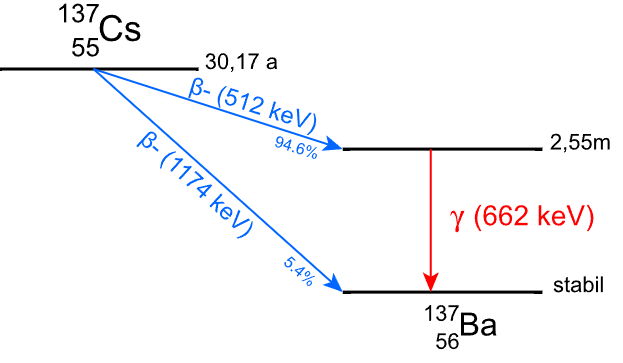
\includegraphics[width=0.45 \textwidth]{latex/images/zerfall.PNG}
    \caption{Eine schematische Darstellung des Zerfalls von $\ce{^{137}Cs}$ zu $\ce{^{137}Ba}$ \protect \cite{leifi}.}
    \label{img:decay}
\end{figure}


\subsection{Licht-Materie-Wechselwirkung}

\noindent
Die Absorption von Strahlung in Materie lässt sich über drei unterschiedliche Prozesse erklären. 
Die Auftrittswahrscheinlichkeit dieser Effekte hängt von der Energie des Photons ab. 
Für unterschiedliche Energiebereiche überwiegen unterschiedliche Effekte.

\noindent
\begin{itemize}
    \item \textbf{Comptoneffekt}\\
        Beim Comptoneffekt trifft das Photon auf ein freies Elektron und vollführt einen inelastischen Stoß. 
        Dabei findet ein Energieübertrag statt, welcher zu einer Wellenlängenänderung beim Photon führt. 
        Des Weiteren ändern sich auch die Ausbreitungsrichtungen des Elektrons und Photons.\\
        Dieser Prozess tritt über das gesamte $\gamma$-Spektrum auf, überwiegt aber für mittlere Energien.
    \item \textbf{Photoeffekt}\\
        Der Photoeffekt tritt am häufigsten bei kleinen bis mittleren $\gamma$-Photonenenergien auf. Bei ihm trifft ein Photon auf ein gebundenes Elektron, 
        überträgt ihm seine gesamte Energie und löst es so aus dem Material. Dieser Effekt tritt nur auf wenn die materialspezifische Austrittsarbeit geleistet wird.
        Die Differenz aus Austrittsarbeit und Photonenenergien erhält das Elektron als kinetische Energie.
    \item \textbf{Paarbildung}\\
        Für die Paarbildung wird eine Photonenenergie von $\SI{1.022}{\mega\electronvolt}$ benötigt, was der Ruhemasse zweier Elektronen entspricht.
        Bei der Paarbildung wandelt ein Photon, welches sich in der Nähe eines anderen Teilchens befindet, seine Energie in ein Elektron-Positron-Paar um.
        Dieser Prozess überwiegt für hohe Energien, wird hier aber nicht betrachtet, da der Zerfall von $\ce{^{137}Cs}$ Photonen mit einer Energie von nur 
        $\SI{662}{\kilo\electronvolt}$ erzeugt, sodass er Effekt nicht auftreten kann.
\end{itemize}


\begin{figure}[H]
    \centering
    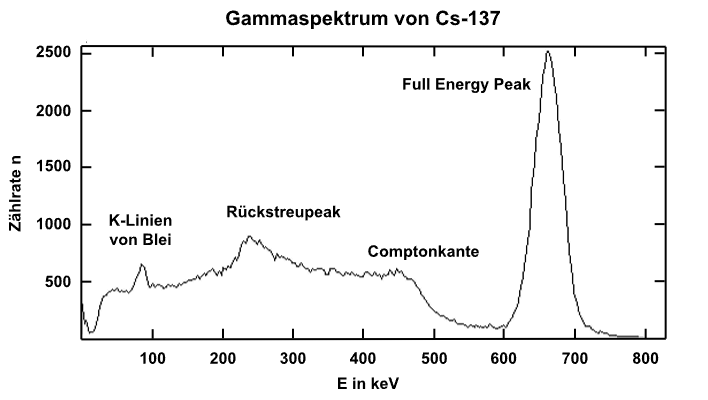
\includegraphics[width=0.7\textwidth]{latex/images/Spektrum.PNG}
    \caption{Das am Szintillationszähler gemessene Intensitätsspektrum für $\ce{^{137}Cs}$ \protect \cite{leifi}.}
    \label{img:spek}
\end{figure}

\noindent
Das Intensitätsspektrum, das hinter der Probe gemessen wird, hat die Form des Spektrums in Abbildung \ref{img:spek}. 
In der Abbildung sind dabei auch die unterschiedlichen Effekte die sich auf das Spektrum auswirken mit ihren Namen gekennzeichnet.\\
Die Comptonkante liegt bei der Energie, bei der der maximale Energieübertrag vom Photon aufs Elektron stattfindet. 
Dies ist also die maximale Energie die durch den Comptoneffekt freigewordene Elektronen besitzen können. 
Vor der Kante befindet sich das Comptonspektrum mit allen möglichen Elektronen-Energien, die durch den Comptoneffekt erzeugt werden können.\\
Der Photopeak wird durch die Elektronen erzeugt, welche über den Photoeffekt aus dem Material gelöst werden und genau die Energie von $\SI{662}{\kilo\electronvolt}$ der Photonen erhalten.\\
Der Rückstreupeak wird von Quanten erzeugt, welche vom Präparat in die entgegengesetzte Richtung bewegen, dann aber an einem anderen Material, wie einer Halterung über den Comptoneffekt wieder in Richtung des Zählers zurück gestreut werden.\\
Die $K$-Linien von Blei entstehen über Anregung von Elektronen in den Blei-Abschirmungen, die dann die Energie der $K$-Linie von Blei besitzen.

